\begin{frame}
    \frametitle{\problemtitle}

    \begin{itemize}
        \item Given an infinite supply of $1\leq n\leq 3\cdot 10^5$ types of bricks, is it possible to
          build a \emph{stable} wall of width $1\leq w\leq 3\cdot 10^5$?
        \item A wall is \emph{stable} when we can alternate two types of rows
          such that the only places two bricks above each other end at the same
          place is at the end of the wall.
        \item If it is possible, also find a suitable layout.
        \item If it is impossible, print ``\texttt{impossible}''.
    \end{itemize}


  \vspace{1em}
  \centering
  
\includegraphics[width=0.46\textwidth]{sample_wa}
  \hfill
  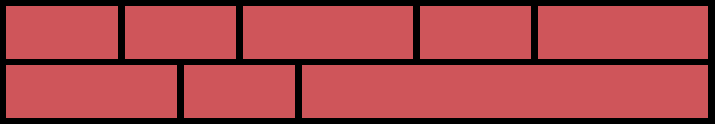
\includegraphics[width=0.46\textwidth]{sample}

  \small
  An unstable (left) and stable (right) wall using the brick types of Sample Input 1.
\end{frame}
